%!TEX root = ../thesis.tex
%*******************************************************************************
%****************************** Third Chapter **********************************
%*******************************************************************************
\chapter{Digitalización de secuencias lineales de proteínas aplicadas al reconocimiento de patrones y modelos predictivos \label{cap3}}

% **************************** Define Graphics Path **************************
\ifpdf
    \graphicspath{{Chapter3/Figs/Raster/}{Chapter3/Figs/PDF/}{Chapter3/Figs/}}
\else
    \graphicspath{{Chapter3/Figs/Vector/}{Chapter3/Figs/}}
\fi

Desarrollar modelos predictivos basados en algoritmos de aprendizaje supervisado, o, la identificación de patrones aplicando técnicas de clustering, son tareas muy relevantes a la hora de trabajar con secuencias de proteínas, ya sea para identificar grupos con características comunes o entrenar modelos predictivos de respuestas de interés. En ambos casos, se requiere el uso de conjuntos de datos altamente informativos y con características numéricas para poder utilizar los métodos implementados en las librerías actuales \cite{pedregosa2011scikit}.

Diferentes metodologías se han implementado, para manipular las variables categóricas en set de datos y lograr su codificación numérica. Enfoques basados en adición de columnas según las categorías o simple transformación empleando representaciones en conjuntos naturales, suelen ser utilizados. No obstante, generan bastante discusión sobre las nuevas representaciones y, a su vez, el hecho de aumentar el número de columnas, conlleva a incrementar las dimensiones del conjunto de datos, provocando efectos negativos en los desempeños de los algoritmos \cite{pedregosa2011scikit}. 

Particularmente, en secuencias de proteínas, se han utilizado las frecuencias de incidencia de los residuos para codificarlos, la cual, pese a su simplicidad, ha resultado ser efectiva en diferentes casos de uso \cite{ozbudak2014protein}. No obstante, este tipo de codificación, no permite explorar el ambiente bajo el cual se encuentran los residuos y tampoco considera el efecto de propiedades fisicoquímicas ni termodinámicas.

En diferentes estudios, los residuos se describen a partir de sus propiedades fisicoquímicas y adicional a ello, se emplea información que permite describir el ambiente del residuo a caracterizar, empleando binarizaciones para describir los residuos cercanos, ya sea por medio del uso de un rango espacial, utilizando modelos o estructuras tridimensionales en donde se representan las coordenadas espaciales de los residuos, o empleando un rango lineal en secuencias lineales de proteínas \cite{capriotti2005mutant2, capriotti2008three}.

Un enfoque basado en las propiedades fisicoquímicas en combinación con la aplicación de transformaciones de Fourier, ha permitido demostrar que ciertos residuos permiten entregar las características asociadas a la propiedad en estudio, además, facilita comprender el aporte del ambiente sobre estos y representa una forma de estudio novedosa para el uso de información de secuencias lineales. Siendo una metodología ampliamente utilizada para identificar residuos que aporten a la propiedad, por medio de la representación de señales asociadas al espacio de frecuencias \cite{veljkovic1985possible, cosic2016analysis, cadet2018application}.

A pesar de ser una metodología interesante a la hora de estudiar secuencias lineales, exhiben problemas notorios sobre la selección de las propiedades relevantes a analizar, ya que, existe un número considerablemente alto de propiedades posibles a utilizar, descritas principalmente en las base de datos AAIndex \cite{Kawashima2000}, y es factible que diferentes familias de proteínas exhiban comportamientos notoriamente no similares y diverjan en cuanto a las propiedades que puedan ser representativas, inclusive, a la hora de estudiar mutaciones en una misma proteína puede que no sólo una propiedad permita su caracterización, si no, que un conjunto pequeño de éstas \cite{cadet2018application}.

En el presente capítulo, se exponen en detalle, diferentes formas de representar secuencias lineales de proteínas, seguido a su vez del planteamiento del uso de transformadas de Fourier para la digitalización de propiedades fisicoquímicas y cómo es posible utilizar éstas para la identificación de patrones en secuencias lineales o el desarrollo de modelos de clasificación/regresión y la exposición de casos de uso en diferentes proteínas de interés. 

\section{Metodologías asociadas a la codificación de variables categóricas}

Diferentes metodologías existen para poder codificar variables categóricas, a su vez, para set de datos de proteínas con secuencias lineales, es factible utilizar sus propiedades fisicoquímicas o frecuencias de residuos. Las principales metodologías usadas a la fecha se exponen a continuación.

\subsection{One Hot encoder}

One Hot encoder, es una de las técnicas más utilizadas a la hora de codificar variables categóricas y se basa principalmente en la adición de columnas con respecto a las categorías existentes en un conjunto de datos \cite{brownlee2017one}.

Dado el vector  $x$ de tamaño $n$ con $m$ categorías, por definición, One Hot encoder agrega al conjunto de datos $m$ columnas, tal que, por cada categoría se adiciona una nueva columna al set de datos. Las nuevas columnas se completan con una binarización de los elementos, indicando si el elemento $x_{i}$ posee la categoría $m_{j}$ con un valor 1 y en caso contrario 0. 

\subsection{Ordinal encoder}

Ordinal encoder, es una simplicación de One Hot encoder, ya que, simplemente codifica las categorías con números en el conjunto $[0, m-1]$. Es decir, sea el vector $x$ de tamaño $n$ con $m$ categorías y sea $M$ el espacio de las posibles categorías con $M = [m_{1}, \cdots, m_{m}]$, y cuya codificación implica el vector $M' = [0, \cdots, m-1]$. $\forall $ elemento que $\in$ a $x$ se obtiene su codificación a partir del elemento $M'(M(m_{i}))$ que corresponde a la codificación de la categoría en el espacio $M$ \cite{pedregosa2011scikit}.

\subsection{Frecuencias de residuos}

Una secuencia lineal de proteína, corresponde a un vector $v$ de tamaño $n$ donde cada elemento corresponde a un residuo que pertenece a la secuencia. El uso de esta información para alimentar modelos de clasificación o regresión conlleva la codificación de sus elementos. Sin embargo, a la hora de utilizar las codificaciones basadas en One Hot Encoder, el conjunto de datos no queda estándar en cuanto a sus dimensiones, ya que, el largo de las secuencias puede variar y a su vez, el número de columnas a agregar corresponde a $n \times 20$ dado a que son $n$ residuos y el espacio muestral $M$ es de tamaño 20 lo que genera un aumento considerable en la cantidad de dimensiones.

Con el fin de poder representar las secuencias lineales de proteínas, se idearon metodologías que consideran la frecuencia de aparición de los residuos en la secuencia, de tal manera, de poder codificarla en un vector de tamaño 20, donde cada elemento representa el número de incidencias del residuo dividido por el largo del vector. Así, cada elemento se encuentra en un rango $[0,1]$ donde 0 indica no incidencia del residuo y 1, incidencia total \cite{ozbudak2014protein}.

El uso de las frecuencias de residuos, es una de las primeras aproximaciones a la codificación de secuencias lineales de proteínas. No obstante, en todos los casos donde han sido utilizadas, se agrega información adicional, que permite comprender diferentes comportamientos y evalúa ciertas propiedades del entorno, razones por las cuales, se recomiendan utilizarlas en conjunto con otros descriptores. 

\subsection{Uso de propiedades fisicoquímicas}

El uso de propiedades fisicoquímicas para describir un residuo, es ampliamente empleado en la generación de descriptores para conjuntos de datos en ingeniería de proteínas \cite{capriotti2005mutant2, capriotti2008three}. Diversos enfoques y modelos han sido construidos o entrenados, contemplando información asociada a componentes termodinámicos del residuo, en particular, a la hora de describir residuos para evaluar cambios en la energía libre, relacionados a efectos en la estabilidad de una proteína \cite{ancien2018prediction, broom2017computational, 1gzp030}.

Se han reportado cerca de 570 propiedades fisicoquímicas que pueden ser utilizadas para describir un residuo en una secuencia lineal de proteínas, almacenadas en la base de datos AAIndex \cite{Kawashima2000}. A su vez, es posible caracterizar estos residuos empleando un conjunto de propiedades estructurales, termodinámicas e inclusive filogenéticas. Es decir, diferentes puntos de vista que permitan describir los residuos pertenecientes a una secuencia. Sin embargo, el hecho de seleccionar qué descriptores son relevantes y cuáles no, radica en un problema de evaluación de características, el cual es común, en el área de la minería de datos. 

Dado al gran conjunto de propiedades existentes y a la diversidad de descriptores que pueden ser utilizados para un conjunto de secuencias lineales de proteínas, es necesaria una selección correcta de las características, las cuales permitan formar set de datos informativos y con una correlación mínima entre sus elementos. 

Contemplando esta problemática, técnicas de reducción de dimensionalidad o análisis de características son las más utilizadas a la hora de seleccionar los descriptores más informativos para un conjunto de datos, siendo ejemplos de esto: Análisis de componentes principales (PCA), Mutual Information, Análisis de correlación y evaluación espacial de características por medio de Random Forest. No obstante, en ocasiones, el conocimiento sobre el problema es un factor relevante a considerar. 

\subsection{Codificación de residuos con adición de información de su entorno}

Adicional a las técnicas explicadas previamente con respecto a las codificaciones existentes, en algunos casos, no sólo basta con una única codificación del residuo, si no, que es relevante adicionar información que puede ser importante para describir los residuos. Normalmente, junto con las codificaciones basadas en propiedades fisicoquímicas, se emplean técnicas que permitan describir el ambiente bajo el cual se encuentre el residuo \cite{masso2008accurate}.

En la gran mayoría de los casos, se adiciona información de los residuos cercanos al residuo de interés, esto depende del tipo de datos bajo el cual se esté trabajando, es decir, si son secuencias lineales o son estructuras de proteínas en formato PDB \cite{capriotti2008three, capriotti2005mutant2}. 

Para el caso de que sean secuencias lineales, sea $s$ secuencia de residuos de tamaño $n$ y sea $r_{i}$ el residuo de interés a evaluar su ambiente. Se crea una ventana de tamaño $n'$ que contempla la cantidad de residuos $r_j$ cercanos al residuo $r_{i}$, de tal manera que se crea un nuevo sub conjunto $s'$ de datos de tamaño $2n'$ con $n'$ residuos a la izquierda y $n'$ a la derecha. El cual normalmente es codificado empleando binarización de elementos, así, en algunas ocasiones, a cada residuo, se le adicionan 20 descriptores que permiten indicar la ausencia o presencia de residuos cercanos a su entorno y el cual se completa con el conjunto de residuos $s'$ \cite{capriotti2008three}.

Cuando se manejan estructuras de proteínas en formato PDB, la codificación y la evaluación del ambiente es similar. Sin embargo, en vez de utilizar una ventana de tamaño $n'$ se utiliza un radio espacial de valor $x$ para el cual, se toma el residuo y se estiman las distancias de los elementos cercanos, ya sea entorno a los carbonos $\alpha$ o a otros elementos. Esto, a diferencia de las secuencias lineales, permite adicionar información sobre las propiedades de distancia, ángulos y conformación de estabilidad por interacciones electrostáticas débiles que pueden generarse a partir de la proximidad de los elementos. No obstante, es una inferencia de su uso y se requieren de diferentes tipos de elementos que permitan caracterizar los eventos asociados al ambiente estructural asociado al residuo \cite{capriotti2008three}.

Actualmente, el uso de codificaciones mediante propiedades fisicoquímicas y el empleo de información adicional basada en descriptores de ambientes, es una de las metodologías más utilizadas a la hora de generar set de datos relacionados a mutaciones. Sin embargo, debido a que sólo se considera distancia, la binarización de los elementos no se ve afectada por sustituciones en residuos lejanos al lugar de ocurrencia, lo que denota la necesidad de idear metodologías que permitan contemplar el aporte completo de residuos a la caracterización de propiedades y cómo sustituciones puntuales afectan enormemente a residuos de interés. Una de las formas en las que se ha intentado dar solución a esta problemática, es modelar las propiedades fisicoquímicas de los residuos de las secuencias, a partir del uso de transformaciones de Fourier y en particular, empleando algoritmos relacionados a dichos conceptos, que aprovechen las ventajas referidas a la manipulación de espacios de frecuencias por sobre elementos temporales.

\section{Transformaciones de Fourier}

Las transformadas de Fourier, corresponden a una transformación matemática que permite analizar una función definida en el espacio tiempo, denominada señal, en sus frecuencias constituyentes. Como característica general, se genera una función definida en el espacio de frecuencias, representada por un valor complejo, en el cual, su módulo corresponde al valor de dicha frecuencia en la función inicial y su coeficiente, corresponde al desfase sinusoidal en la frecuencia \cite{sneddon1995fourier}.

Sea $f$ una función definida en el espacio tiempo, representando una señal, integrable Lebesgue, su transformada se define como $f: \mathbb{R} \to \mathbb{C}$, asociada a una frecuencia, denotada por $\hat{f}$, la cual se expresa como:

\begin{equation}
	\hat{f}(\xi) = \int_{-\infty}^{+\infty} f(x)e^{-2\pi i x \xi} dx
	\label{tran1}
\end{equation}

Donde $\xi$ corresponde a un número real y $x$ representa al tiempo. A partir de \ref{tran1}, se puede definir la transformación inversa

\begin{equation}
	f(x) = \int_{-\infty}^{+\infty} \hat{f}(\xi) e^{-2\pi i x \xi} d\xi
	\label{tran2}
\end{equation}

Tanto \ref{tran1} y \ref{tran2}, corresponden a funciones con distribución continua. De manera similar, es posible definir las transformada de Fourier y su inversa, en el espacio de distribuciones discretas, en donde, sólo se considera un segmento muestral finito del conjunto de datos continuos para reconstruir el espectro de frecuencias \cite{rao2014discrete}. Dado esto, la transformada de Fourier discreta se define como:

\begin{equation}
	X_k = \sum_{n=0}^{N-1} x_n e^{-\dfrac{2\pi i}{N} kn}\ \ \  \forall\  k \in [0, N-1]
\end{equation} 

Donde $N$ representa a una secuencia de números complejos $x_0, \cdots, x_{N-1}$. Se define la transformada discreta inversa de Fourier como:

\begin{equation}
	x_n = \dfrac{1}{N} \sum_{k=0}^{N-1} X_k e \dfrac{2\pi i}{N} kn \ \ \ \forall \ n \in [0, N-1]
\end{equation}

Las transformadas de Fourier han sido utilizadas en diferentes campos de investigación, tales como: física, teoría de números, procesamiento de señales, propagación de ondas, óptica, etc. Siendo el análisis armónico, la rama matemática encargada de este tipo de estudios.

A partir de lo anterior, debido a los diferentes empleos que puede tener esta transformada, nace la necesidad de resolver de manera eficiente esta función, para ello nacen diferentes algoritmos, dentro de los cuales, el principal se conoce como Transformada rápida de Fourier (FFT por sus siglas en inglés).
 
\subsection{Transformada rápida de Fourier (FFT)}

La transformada rápida de Fourier (FFT por sus siglas en inglés), es un algoritmo que permite encontrar solución a una DFT con una disminución en la complejidad. Esto es, al resolver el problema directamente desde la DFT, se presenta una complejidad $O(N^2)$, en cambio, al utilizar FFT, se obtiene una complejidad de $O(N\log N)$ \cite{welch1967use}.

La idea general del algoritmo fue propuesto por Cooley \cite{cooley1970fast}. Dentro de sus particularidades, es que debido a la subdivisión en $N$ transformadas de menor complejidad a resolver, donde $N$ se compone de $n_1$ y $n_2$, se requiere que el conjunto de muestras, presente un tamaño del orden $2\cdot 2^n$, es decir, una potencia de 2. A pesar de que dicho algoritmo es uno de los más comunes para la resolución de transformadas de Fourier, no es el único, siendo algunos: Prime-factor FFT algorithm \cite{kolba1977prime}, Bruun's FFT algorithm, Rader's FFT algorithm, Bluestein's FFT algorithm, and Hexagonal Fast Fourier Transform \cite{cui2005some}.

Las definiciones matemáticas del proceso, se realizaron por Peter D. Welch en \cite{welch1967use}, explicando la formulación del problema y las demostraciones de la solución. 

La división que se genera en el algoritmo FFT propuesto por Cooley \cite{cooley1970fast}, se basa en el uso de radix-2 DIT, esto es, la división de una DFT de tamaño $N$ en dos DFT de tamaño $N/2$ de manera recursiva.

De manera general, se estiman las DFT de los pares e impares por separado ($x_{2m}$ y $x_{2m+1}$, respectivamente), para luego combinarlas y estimar la DFT del espacio completo Debido a esta subdivisión recursiva en pares, se requiere un número de componetes en potencia de 2. Normalmente, se adicionan elementos para poder cumplir con dicha condición, comúnmente, se utiliza \textit{zero-padding} \cite{muquet2002cyclic}, para satisfacerlo.

Matemáticamente, las DFT de los componentes pares e impares y su combinación se obtiene a partir de:

\begin{equation}
	X_{k} = \sum_{m=0}^{N/2 -1} x_{2m} e ^{-\dfrac{2\pi i}{N}2mk}\ +\ \sum_{m=0}^{N/2 -1} x_{2m+1} e ^{-\dfrac{2\pi i}{N}(2m+1)k} 
	\label{tran3}
\end{equation}  

Donde el primer componente denota los elementos pares $E_k$ y el segundo componente los impares $O_k$ en la ecuación \ref{tran3}, respectivamente.

Un esquema representativo de los pasos a seguir en el algoritmo, la utilización del radix-2 DIT y cómo se obtienen las DFT para luego combinarlas se expone en la Figura \ref{algo}.
\begin{figure}[!h]
	
	\centering
	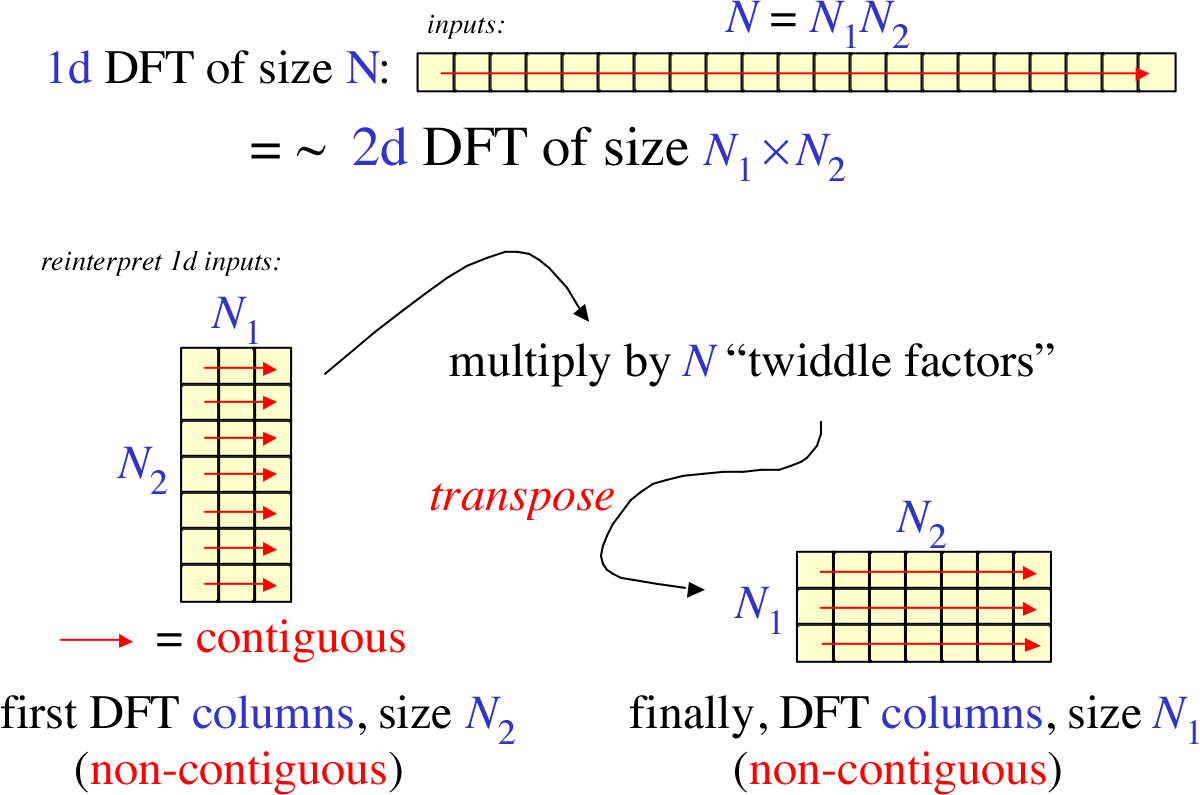
\includegraphics[scale = .6]{algorithm.png}
	\caption{Esquema representativo de los pasos asociados al algoritmo FFT, desarrollado por Cooley \cite{cooley1970fast}}
	\label{algo}
\end{figure}

\subsection{Uso de Transformadas de Fourier en digitalización de propiedades fisicoquímicas}

Diferentes enfoques han sido evaluados mediante el empleo del uso de las transformadas de Fourier en el estudio de secuencias lineales de proteínas y DNA, en particular, para el estudio de propiedades fisicoquímicas y la identificación de residuos claves asociados a peacks visuales en el espectro de frecuencia \cite{veljkovic1985possible, cosic1987prediction}. 

El uso frecuente de la digitalización, se centra principalmente en la codificación de una secuencia lineal de proteínas, en muchos casos, ha sido utilizado el potencial de interacción con electrones (PEII), ya que se han expuesto correlaciones con propensiones de moléculas orgánicas, relacionadas con toxicidad, actividad de antibióticos, carcinogenecidad, etc. \cite{veljkovic1985possible, cosic1994macromolecular, cosic1987prediction} y a partir de dicha codificación, digitalizarla para el posterior estudio de la análisis de señales.

Dichos estudios de frecuencia de señales, son componentes de modelos asociados al reconocimiento de resonancias (RRM por sus siglas en inglés), los cuales han sido estudiados en diferentes problemas del área médica, reconocimiento de Hot-spots, etc., y, en particular, enfocados en el estudio de mutaciones en proteínas \cite{cosic1994macromolecular, cosic2016analysis, cosic1987prediction}. 

Un enfoque común, asociado al estudio de señales y modelos RRM, consiste en, a partir de la secuencia lineal de residuos, emplear PEII para codificarla, a partir de su codificación, se aplica FFT como método de digitalización, para así, obtener el espectro de frecuencia y hacer los análisis de señales correspondientes \cite{veljkovic1985possible, cosic1994macromolecular, cosic2016analysis, cosic1987prediction}.

No obstante, existen otros enfoques, en donde se ha utilizado la digitalización de las propiedades fisicoquímicas como método de generación de atributos para set de datos, los cuales son sometidos a entrenamiento de predicciones, entregando medidas de desempeño satisfactorias, según los autores \cite{cadet2018application}. Sin embargo, la selección de las propiedades fisicoquímicas es arbitraria y sólo se considera la propiedad más informativa, no considerando el uso de combinaciones lineales o correlaciones entre las propiedades existentes.

Uno de los puntos relevantes, es que a partir de un conjunto de espectros de frecuencia, es posible generar un consenso y a su vez, identificar residuos relevantes al espectro y que contribuyen de manera significativa en los peaks, así como también la generación de espectros consenso a partir de secuencias diferentes, entregando uno de los principales planteamientos. \textit{Un mismo espectro de frecuencia, está asociado a una propiedad o una funcionalidad}, lo cual fue testeado en trabajos como \cite{veljkovic1985possible}. 

Esto último, lo hace una de las ventajas más relevantes para el estudio de mutaciones o reconocimiento de patrones. Sin embargo, la generalización del método ha impedido que se utilice con un mayor impacto, sólo siendo empleado en los estudios nombrados previamente. No obstante, las posibilidades de encontrar patrones o permitir modelar sistemas complejos, además de aplicar las propiedades del estudio de señales a dichos entornos de secuencias, y, las posibilidades que este método entrega para el análisis de estructuras lineales, lo hace una propuesta interesante y novedosa, que merece un esfuerzo estudiarla y aplicarla durante este trabajo de tesis.

\section{Clustering}

Clustering se define como un método de aprendizaje no supervisado, en el cual se cuenta con un conjunto de datos que representan a una muestra y en base a ésta, se trata de obtener grupos de objetos, denominados clusters \cite{jain1999data}.

Los clusters deben cumplir con dos características fundamentales:

\begin{itemize}
	\item Los objetos que pertenezcan a un mismo clúster deben ser bastante homogéneos entre ellos.
	\item Entre los clústers debe existir un alto grado de heterogeneidad.
\end{itemize}

Los métodos de clustering tratan, fundamentalmente, de resolver el siguiente problema: Dado un conjunto de $N$ individuos, caracterizados por la información de $n$ variables $X_{j}$ con $j$ entre $1,..,n$, se plantea el reto de ser capaces de agruparlos de manera que los individuos pertenecientes a un grupo (cluster), dada la información disponible, sean tan similares entre sí como sea posible, siendo los distintos grupos entre ellos tan disimilares como sea posible.

Básicamente, el análisis constará de un algoritmo de clustering que permitirá la obtención de una o varias particiones, de acuerdo con los criterios establecidos.

\subsection{Algoritmos de Clustering}

Existen diversos algoritmos de clustering, cada uno con características que los diferencian, los cuales, pueden ser aplicados a diversos casos, dependiendo de las características de los datos de entrada, es decir, de la geometría de estos datos. Sin embargo, esta representación se basa principalmente en el uso de matrices, donde cada fila representa un ejemplo y cada columna el valor de un atributo o rasgo cualitativo para dicho ejemplo.

Los principales algoritmos de aprendizaje no supervisado se resumen en la Tabla \ref{cuadroResumen} se expone un resumen de las características de cada algoritmo expuesto, la escalabilidad que poseen, las distancias que ocupan, los casos de uso y los parámetros que poseen.

\begin{table}[]
	\centering
	\begin{tabular}{|l|l|l|l|l|}
		\hline
		\multicolumn{5}{|c|}{\textbf{Tabla resumen de Algoritmos de Aprendiza No Supervisado}}                                                                                                                                                                                                                                                                                                                                                                                                                                          \\ \hline
		\textbf{Algoritmo}                                                                  & \textbf{Parámetros}                                                                       & \textbf{Escalabilidad}                                                                                  & \textbf{Usos}                                                                                                                                 & \textbf{Métrica usada}                                                              \\ \hline
		\textbf{K-Means}                                                                    & \begin{tabular}[c]{@{}l@{}}Número de \\ clúster\end{tabular}                              & \begin{tabular}[c]{@{}l@{}}Muchas muestras, \\ mediana cantidad\\ de clúster.\end{tabular}              & \begin{tabular}[c]{@{}l@{}}De propósito\\ general, la \\ geometría plana, \\ no demasiados \\ grupos\end{tabular}                             & \begin{tabular}[c]{@{}l@{}}Distancia entre\\ puntos\end{tabular}                    \\ \hline
		\textbf{\begin{tabular}[c]{@{}l@{}}Affinity \\ propagation\end{tabular}}            & preferencia                                                                               & \begin{tabular}[c]{@{}l@{}}No escalable con \\ n ejemplos\end{tabular}                                  & \begin{tabular}[c]{@{}l@{}}Muchos clúster, \\ tamañode clúster \\ desigual, \\ geometría no \\ plana\end{tabular}                             & \begin{tabular}[c]{@{}l@{}}Distancia\\ gráfica\end{tabular}                         \\ \hline
		\textbf{Mean-shift}                                                                 & bandwidth                                                                                 & \begin{tabular}[c]{@{}l@{}}No escalable con \\ n ejemplos\end{tabular}                                  & \begin{tabular}[c]{@{}l@{}}Muchos clúster, \\ tamañode clúster \\ desigual, geometría \\ no plana\end{tabular}                                & \begin{tabular}[c]{@{}l@{}}Distancia entre\\ puntos\end{tabular}                    \\ \hline
		\textbf{\begin{tabular}[c]{@{}l@{}}Ward \\ hierarchical \\ clustering\end{tabular}} & \begin{tabular}[c]{@{}l@{}}Número de \\ clúster\end{tabular}                              & \begin{tabular}[c]{@{}l@{}}Mucha cantidad \\ de ejemplos y de \\ clusters\end{tabular}                  & \begin{tabular}[c]{@{}l@{}}Cualquier clúster, \\ es posible \\ conección de \\ constraints\end{tabular}                                       & \begin{tabular}[c]{@{}l@{}}Distantia entre\\ puntos\end{tabular}                    \\ \hline
		\textbf{\begin{tabular}[c]{@{}l@{}}Agglomerative \\ clustering\end{tabular}}        & \begin{tabular}[c]{@{}l@{}}Número de \\ clúster, tipo de \\ unión, distancia\end{tabular} & \begin{tabular}[c]{@{}l@{}}Mucha cantidad\\ de ejemplos y de\\ clusters\end{tabular}                    & \begin{tabular}[c]{@{}l@{}}Muchos clusters, \\ posiblemente \\ restricciones de \\ conectividad, \\ distancias \\ no euclidianas\end{tabular} & \begin{tabular}[c]{@{}l@{}}Cualquier \\ distancia pairwise\end{tabular}             \\ \hline
		\textbf{DBSCAN}                                                                     & tamaño vecino                                                                             & \begin{tabular}[c]{@{}l@{}}Mucha cantidad \\ de ejemplos, \\ mediana\\ cantidad de clúster\end{tabular} & \begin{tabular}[c]{@{}l@{}}Geometría no plana, \\ tamaños de clusters \\ distintos\end{tabular}                                               & \begin{tabular}[c]{@{}l@{}}Distancia entre\\ puntos vecinos\end{tabular}            \\ \hline
		\textbf{\begin{tabular}[c]{@{}l@{}}Gaussian \\ mixtures\end{tabular}}               & variado                                                                                   & No escalable                                                                                            & \begin{tabular}[c]{@{}l@{}}Geometría plana, \\ bueno para la \\ estimación de la \\ densidad\end{tabular}                                     & \begin{tabular}[c]{@{}l@{}}Distancia \\ Mahalanobis para\\ los centros\end{tabular} \\ \hline
		\textbf{Birch}                                                                      & \begin{tabular}[c]{@{}l@{}}branching, \\ umbral\end{tabular}                              & \begin{tabular}[c]{@{}l@{}}Alto número de\\ clúster y ejemplos\end{tabular}                             & \begin{tabular}[c]{@{}l@{}}Largo set de datos, \\ eliminación valores \\ atípicos, \\ reducción de datos\end{tabular}                         & \begin{tabular}[c]{@{}l@{}}distancia \\ euclidiana\\ entre puntos\end{tabular}      \\ \hline
	\end{tabular}
	
	
	\caption{Cuadro resumen de algoritmos de aprendizaje supervizado}
	\label{cuadroResumen}
\end{table}

\subsection{Métodos de clustering empleando estructuras de grafos}

Un grafo, es una estructura de datos compleja, que se compone de nodos y aristas, los nodos, son aquellos que representan la información y las aristas, permiten enlazar nodos. Existen diferentes tipos de representaciones, los cuales se basan en cómo fluye la información, encontrándose grafos dirigidos y no dirigidos. Los primeros, tienen una dirección entre un nodo $A$ y $B$, la cual puede indicar diferentes comportamientos, por ejemplo, si los nodos representan genes, es posible mencionar que $A$ regula a $B$. En el caso de grafos no dirigidos, no existe la relación expuesta previamente.

Matemáticamente, es posible definir las estructuras de gráfos, como un par de conjuntos $G =(V,E)$, donde $V$ es el conjunto de vértices y  $E$ representa las aristas del grafo. En un grafo no dirigido, cada arista es un par no ordenado ${v,w}$. En un grafo dirigido, las aristas son pares ordenados. Los vértices $v$ y $w$ son llamados puntos finales de una arista. La cantidad de aristas $|E|=m$ es el tamaño del grafo. En un grafo ponderado, una función $\omega: E \rightarrow \mathbb{R}$ es definida la cual pondera cada arista.

Existen diversas utilidades que pueden ser expuestas usa para modelar problemas reales como redes de computadoras, redes sociales y estructuras de proteínas, entre otros. 

Otro de los puntos que pueden ser explotados en un grafo, es el hecho de generar clustering o identificación de comunidades, las cuales se definen como un conjunto de nodos, los que están fuertemente conectados entre sí y débilmente enlazados con otros elementos \cite{fortunato2012community}. Los principales uso de las comunidades o sub grafos, corresponden a identificación de patrones con comportamientos particulares desde un punto de vista diferente a cómo lo hacen los métodos de aprendizaje no supervisado. Dentro de los diferentes algoritmos que permiten efectuar dicha búsqueda, se encuentran: Fast Greedy, Edge Betweenness, Cluster Walktrap, Leading eigenvector, Louvain, Infomap, dentro de los principales \cite{newman2004detecting}.
 
De manera análoga a las medidas de desempeño para la evaluación de los clustering empleadas en algoritmos de aprendizaje no supervisado, existe el concepto de modularidad \cite{Newman8577}, el cual permite evaluar la disgregación de los elementos y la densidad de las comunidades. Donde un valor de 0.35 es aceptado como comunidades bien definidas.

\section{Hipótesis}

Dada la problemática existente sobre cómo representar conjuntos de secuencias lineales con el fin de poder desarrollar modelos de clasificación/regresión o identificación de patrones asociados a propiedades fisicoquímicas. Y, en consideración de los diferentes usos que entrega las transformadas de Fourier, se plantea la hipótesis de este capítulo.

\begin{center}
	\textit{La codificación de secuencias lineales empleando espectros de Fourier, basados en las
		propiedades fisicoquímicas de los residuos de la proteína, permite generar descriptores
		que facilitan el aprendizaje de predictores de variantes enfocados a diferentes respuestas de
		interés. A su vez, es posible correlacionar propiedades fisicoquímicas o funciones con propiedades de los 
		espectros de frecuencia}
\end{center}

Si bien, en el planteamiento de la hipótesis se exponen dos preguntas, la interrogante en sí, se centra a los posibles usos que pueda tener los espectros de frecuencia en el estudio de variantes, identificación de patrones, residuos relevantes, etc.

\section{Objetivos}

En base a la hipótesis planteada y con el fin de responder a los planteamientos e interrogantes expuestas. Se detallan el objetivo general y los objetivos específicos.

\subsection{Objetivo general}

Diseñar e implementar metodología de codificación y digitalización de propiedades fisicoquímicas en secuencias lineales de proteínas, empleando transformadas rápidas de Fourier, con el fin de poder ser utilizadas en identificación de patrones por medio de técnicas de clustering o desarrollo de predictores basados en algoritmos de aprendizaje supervisado.

\subsection{Objetivos específicos}

A partir del objetivo general, nacen los siguientes objetivos específicos.

\begin{enumerate}
	
	\item Preparar, manipular e implementar módulos de consultas para la base de datos de propiedades fisicoquímicas asociadas a la base de datos AAindex \cite{Kawashima2000}.
	
	\item Diseñar e implementar, metodologías de codificación de propiedades fisicoquímicas y selección de las más representativas, por medio de técnicas de reducción de dimensionalidad y selección de características, descritas a través de espectros de frecuencia.
	
	\item Implementar y validar modelos de clasificación/regresión para evaluación de análisis de estabilidad de variantes según descriptores basados en espectros de frecuencia de propiedades fisicoquímicas.
		
	\item Diseñar, implementar y caracterizar grupos obtenidos a partir de algoritmos de aprendizaje no supervisados, considerando como descriptores los espectros de frecuencias asociados a las propiedades fisicoquímicas.
	
\end{enumerate}

\section{Metodología}

Con el fin de poder cumplir con el objetivo general planteado y los objetivos específicos, se expone a continuación la metodología diseñada. Se consideran diferentes etapas dentro de las cuales se destaca la codificación, entrenamiento de modelos, aplicación de clustering e identificación de residuos como patrones de señales dentro del espectro de frecuencia.

A continuación de exponen las diferentes etapas asociadas al proceso.

\subsection{Identificación y selección de propiedades fisicoquímicas}

El uso de la base de datos AAIndex, contempla trabajar con 566 propiedades que describen a un residuo, dentro de las cuales, existen altas correlaciones entre diferentes propiedades, ya que, evalúan el mismo concepto. Pero, empleando técnicas o metodologías diferentes. Razón por la cual, es necesario evaluar cuáles son las propiedades que pueden ser utilizadas, con el fin de no generar redundancia de información.

A partir de lo anterior, se emplean estructuras de grafos no dirigidos, en los cuales, los nodos representan la propiedad y las aristas corresponden a si existe una alta correlación entre la propiedad $A$ y $B$. Se destaca que dicha correlación se mide con respecto al coeficiente de Pearson y sólo se considerará altamente correlacionados si dicho índice es sobre 0.9. Una vez creado el nodo, se aplicarán diferentes algoritmos de identificación de comunidades y se evaluará la modularidad de estos, a través de la cual, se seleccionarán las con mayor índice.

Esto último, permite generar grupos de propiedades cuya característica principal es que presentan alta correlación entre ellos, dado esto, si se tienen $n$ comunidades, es posible representar una secuencia lineal a partir de cualquier propiedad seleccionada de cada comunidad $n_i$. De esta forma, se reduce la dimensión del espacio muestral.

\subsection{Codificación de secuencias lineales}

La codificación de secuencias lineales, se basa en el uso de propiedades fisicoquímicas representativas de la secuencia, las cuales se obtienen a partir de la base de datos AAindex\cite{Kawashima2000} y son seleccionadas de manera aleatoria con respecto a las comunidades identificadas a través de la correlación de dichas características desde las estructuras de grafos generadas.

Un esquema representativo del proceso, se observa en la Figura \ref{cap3:fig1}, en la cual, se detallan los diferentes pasos a seguir para generar la codificación correspondiente y obtener los espectros de frecuencias asociados a cada propiedad fisicoquímica.

\begin{figure}[!h]
	
	\centering
	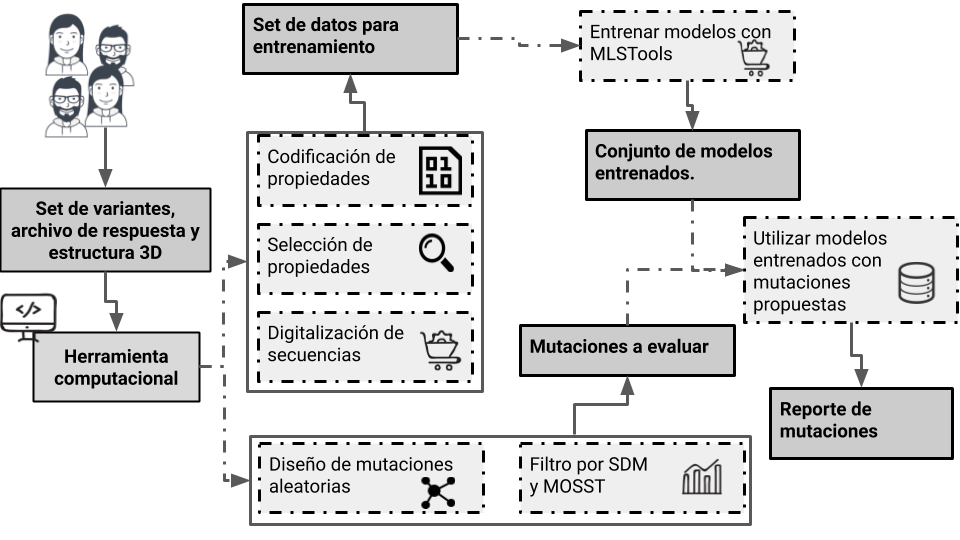
\includegraphics[scale=.4]{fig1.png}
	\caption{Esquema representativo, metodología de digitalización de secuencias.}
	\label{cap3:fig1}
\end{figure}

En una primera instancia, se toma la secuencia y por cada residuo se crea un vector de tamaño $n$ el cual representa el número de propiedades fisicoquímicas a considerar a partir de las comunidades generadas. De esta forma, se crea una matriz de tamaño $r \times n$ donde $r$ representa la cantidad de residuos en la secuencia.


A partir de dicha matriz, técnicas de reducción de dimensionalidad y selección de características son implementadas, utilizando lenguaje de programación Python y la librería scikit-learn \cite{pedregosa2011scikit}, con el fin de seleccionar cuáles son las propiedades más representativas y qué porcentaje de la varianza permiten explicar.

Dado el conjunto de propiedades seleccionadas, se implementarán rutinas basadas en lenguaje de programación Matlab, las cuales reciben el conjunto inicial de datos, en una primera instancia, aplica \textit{zero-padding} con el fin generar vectores de tamaño de potencia de $2\cdot2^n$, requisito para la aplicación de FFT. A partir de esto, cada columna en el conjunto de elementos, se digitaliza por medio del uso de la transformada rápida de Fourier (FFT) y se obtienen los espectros de frecuencias para cada propiedad fisicoquímica seleccionada previamente.

De esta forma, por cada secuencia, se obtiene un conjunto de espectros de frecuencia, asociados a la digitalización de las propiedades fisicoquímicas seleccionadas mediante técnicas de selección de características.

\subsection{Caracterización del espectro de frecuencias}

Dado el conjunto de espectros de frecuencia generado para las secuencias lineales, es necesario extraer información relevante de estos con el fin de caracterizarlo, para ello, se plantean diferentes metodologías con el fin de poder generar los conjuntos de entrenamientos, y, a partir de estos, implementar los modelos predictivos propuestos. Es importante mencionar, que dichos patrones también pueden ser utilizados como método de reconocimiento de residuos relevantes en las variantes, ya que, si se aplica la transformada inversa de Fourier, es posible la identificación de los elementos que participan en algún peak del espectro \cite{veljkovic1985possible}.

Tomando esto en consideración, se plantean diversas metodologías que serán implementadas para llevar a cabo la caracterización del espectro. Un punto relevante, es el hecho de que al ser una etapa exploratoria, será necesario evaluar cuál es la mejor, a la hora de aplicarla en entrenamiento de modelos predictivos. Cada una de las cuales, se explica a continuación.

\subsubsection{Diferencias espectrales}
 
Sea $f_i(wild)$ el espectro de frecuencia de la proteína no mutada para la propiedad $i$ y $f_i(mut_{j})$ el espectro de frecuencia para la mutante $j$. Se define el espectro diferencial como la resta de $f_i(wild)$ y $f_i(mut_{j})$.

Ya que se tendrán $j$ mutantes, existirán $j$ diferencias espectrales, a partir de las cuales, se emplearán para formar conjuntos de datos y entrenar modelos predictivos.

Uno de los puntos importantes a destacar, radica en el hecho de es posible identificar variaciones positivas y negativas, lo cual puede influir de diferentes formas en la propiedad y por consecuencia, en la función o respuesta asociada a evaluar.

\subsubsection{Binarización de diferencias espectrales}

A partir de las diferencias espectrales expuestas en el punto anterior, es posible desarrollar distribuciones de las diferencias de los espectros, de tal manera, que se apliquen test estadísticos para la identificación de outliers en la muestra, con un nivel de significancia $\alpha$.

Dado esta identificación, se considera el conjunto de elementos y se codifica con respecto a si es un outlier positivo, negativo o se encuentra dentro del rango normal de distribución. De esta forma, por cada espectro, se forma un vector binarizado, dando origen a una matriz de espectros codificados en base a la significancia de su diferencia.

Dicha matriz se utiliza para el entrenamiento de modelos predictivos, a su vez, esta matriz podría ser representada en un heat map, con el fin de poder identificar zonas en las que exista una mayor densidad de puntos con tendencia hacia un tipo de outlier.

\subsubsection{Identificación de zonas en el espacio espectral}

De manera visual, el espectro de frecuencia en sí, es informativo, ya que, permite identificar zonas en las que existe un peak, las cuales reflejarían una característica correlacionada con la función \cite{vijayakumar1998electrostatic}. A su vez, si se considera la diferencia espectral, ésta, permitirá identificar cómo fue la variación con respecto a la proteína inicial, de tal manera que, una distribución uniforme con valor 0 debiese pertenecer a variantes que no afecten los valores de la propiedad en sí, mientras que, variaciones importantes, serán detectadas en zonas específicas de la distribución. A su vez, al binarizar la distribución de diferencias, es posible visualizar estas tendencias. 

Con el fin de reconocer de manera automática dichas zonas, se trabaja con las distribuciones discretas de los espectros binarizados, obtenidos previamente, para las cuales, se diseñará e implementará un algoritmo de detección de cambios en la distribución, tal que, permita ir marcando por zonas en donde se exhiba un cambio positivo, negativo o neutro. 

A su vez, sería interesante de estudiar, o, identificar las variantes generadas y sus correspondientes efectos y ver cómo se clasifican en estas zonas, ya que, podría ser identificable, zonas en el espectro, que conllevan una alteración negativa para una proteína, tal que, se podría identificar, cuáles son los residuos o posiciones que más afectan a un cambio negativo en la proteína. 

Con los diferentes puntos expuestos previamente, se generan distintas caracterizaciones, que permiten describir el espectro y generar el conjunto de datos, el cual será utilizada para el entrenamiento de modelos predictivos.

\subsection{Implementación de modelos de clasificación/regresión para análisis de variantes}

Uno de los objetivos de la codificación de secuencias lineales, es evaluar si el conjunto de espectros de frecuencia para un grupo de variantes, puede ser utilizado como características para generar set de datos y entrenar modelos a partir de estos.

Con esto en mente y apoyados en los conjuntos de datos utilizados para la generación de descriptores basados en propiedades termodinámicas y filogenéticas, expuestos en el capítulo \ref{cap2}, se desarrollarán modelos de clasificación para la evaluación de la estabilidad de proteína y modelos de regresión para la predicción del cambio en la energía libre provocado por los residuos.

En la Figura \ref{cap3:fig3}, se expone un esquema representativo asociado a los pasos a seguir para el desarrollo de los modelos.

\begin{figure}[!h]
	
	\centering
	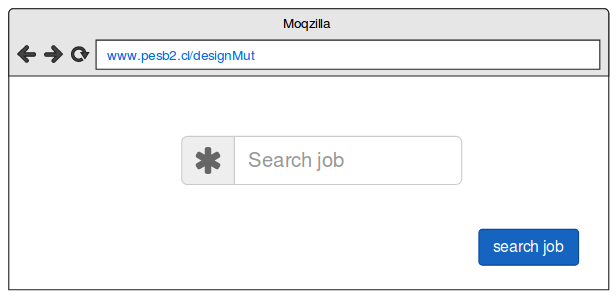
\includegraphics[scale=.4]{fig3.png}
	\caption{Esquema representativo, metodología de clustering se secuencias por medio de espectros de frecuencias basados en propiedades fisicoquímicas.}
	\label{cap3:fig3}
\end{figure}


En una primera instancia, se necesita preparar el conjunto de datos, para ello, se considerarán la secuencia original de la proteína y serán generadas las variantes con respecto a la mutación reportada. De esta forma se creará un conjunto de datos basados en una variante y la respuesta asociada, lo cual corresponde a las diferencias de energía libre que provoca la sustitución del residuo o clasificación de estabilidad.

Al conjunto de secuencias generado, se aplicará la codificación de las propiedades fisicoquímicas, a partir de la información existente en la base de datos AAindex.

Posterior a ello, se seleccionarán las propiedades más informativas y se generará la digitalización de éstas, empleando la metodología descrita en el punto anterior. La selección de las características se basa en un consenso con respecto a las incidencias de cada propiedad en cada secuencia, esto es, dado a que se seleccionan $p$ propiedades por cada secuencia, es posible que diferentes secuencias, presente distintas propiedades. Por lo tanto, se seleccionarán aquellas propiedades que presenten mayor incidencia en el conjunto de secuencias, ya que éstas, serán las más representativas del conjunto completo. 

Una vez se tenga el conjunto de espectros caracterizado, modelos predictivos serán entrenados aplicando algoritmos de aprendizaje supervisado al set de datos de espectros de frecuencia. Se utilizarán las medidas de desempeño expuestas en el capítulo \ref{cap2}. Los modelos serán validados mediante validación cruzada con un valor de $k=10$, con el fin de evaluar el sobreajuste. 

Finalmente, los resultados a obtener a partir de descriptores basados en espectros de frecuencia, serán comparados con los obtenidos en la fase de exploración de la metodología expuesta en el capítulo 2. Esto con el fin de determinar, qué metodología o caracterización de datos, permite entregar un modelo con mejor desempeño o características deseables. 

Es importante mencionar que, los modelos que se obtengan a partir de la digitalización de propiedades fisicoquímicas, pueden presentar  performance inferior a los modelos a obtener aplicando la metodología del capítulo \ref{cap2}. Sin embargo, si el desempeño es alto, sería suficiente para responder la pregunta planteada. Si son bajos o azarosos, implica que se requiere un mayor refinamiento a la metodología, o, que simplemente el conjunto de datos presenta problemas para entrenar modelos, razón por la cual, debiese descartarse. 

\subsection{Aplicación de técnicas de clustering sobre espectros de frecuencia}

Uno de los supuestos más relevantes asociados al uso de la digitalización y las propiedades fisicoquímicas como descriptores de secuencias lineales, es el hecho de que, proteínas con una misma función, presentan un espectro de frecuencia similar \cite{veljkovic1985possible}. 

Esto, hace pensar que, para un conjunto de secuencias desconocidas, dada una selección de propiedades fisicoquímicas, a la hora de aplicar técnicas de clustering, empleando algoritmos de aprendizaje no supervisado, serán agrupadas de tal forma, que, los espectros de frecuencia en cada grupo presenten similitudes entre ellos, basados en propiedades estadísticas o por medio de análisis cross-espectral.
 
Con el fin de corroborar este supuesto, además de demostrar que el uso de descriptores basados en espectros permite una agrupación de elementos correlacionados con alguna propiedad, en la Figura \ref{cap3:fig2} se expone la metodología planteada.

\begin{figure}[!h]
	
	\centering
	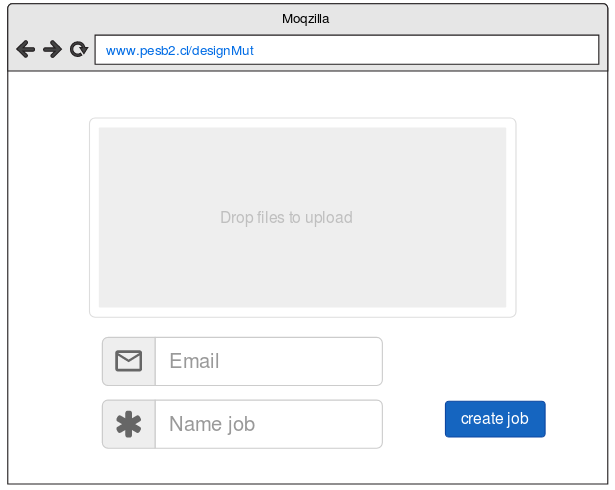
\includegraphics[scale=.4]{fig2.png}
	\caption{Esquema representativo, metodología de clustering se secuencias por medio de espectros de frecuencias basados en propiedades fisicoquímicas.}
	\label{cap3:fig2}
\end{figure}

En una primera instancia, se deberá identificar cuáles son las secuencias de interés, para ello, se trabajarán con diferentes secuencias lineales y variantes asociadas a ellas, principalmente de enzimas, con alguna propiedad característica, proteínas comunes de interés con mutaciones reportadas, etc. La descarga de éstas, se realizará desde diferentes bases de datos, en particular desde Brenda \cite{schomburg2004brenda}, para el caso de las enzimas, Protherm \cite{bava2004protherm} para otras propiedades de interés, relacionadas a estabilidad. 

Es importante mencionar, que no se quiere asociar o reconocer qué efecto causa la mutación. Si no, probar que, proteínas con similar función, tendrán un espectro de frecuencia con características comunes. Es por ello, que la propiedad se conoce de antemano. Sin embargo, también se evaluará si es posible la generación de grupos donde la mutación afecte negativa y positivamente a la estabilidad en proteínas, utilizando para esto, el conjunto de set de datos expuestos en el capítulo \ref{cap2}.

Una vez se tengan las secuencias, se aplicará la codificación de diferentes propiedades fisicoquímicas y a su vez, se digitalizará cada una de éstas. Es importante mencionar, que no se seleccionarán propiedades específicas ya que, puede que las más representativas o informativas no necesariamente generen conjuntos de datos agrupados con el mismo patrón de espectro de frecuencia. 

Esto implica, que se generarán $n$ espectros de frecuencia por cada secuencia y para cada propiedad se aplicarán técnicas de clustering, esto con el fin de determinar si aparecen grupos con misma propiedad conocida, correspondientes a las $n$ propiedades descritas en AAindex. Lo anterior, permitirá evaluar si proteínas con misma funcionalidad, o mismo plegamiento, o, alguna característica en común, quedan agrupadas.

Finalmente, una vez se tengan estos grupos, se realizará la etapa de análisis, caracterización e identificación de patrones. Esto es, en base a la información conocida que se tiene del conjunto de proteínas, evaluar si los grupos formados presentan algo en común, ya sea, propiedades fisicoquímicas, plegamiento, actividad, funcionalidad, etc. 

Esto permitirá evaluar si los espectros de frecuencia, permiten agrupar secuencias con características o patrones en común y si son informativas para dicho objetivo. Se destaca además, que esto implica una fase exploratoria y es incierto lo que pueda resultar. Si bien se postuló las correlaciones entre espectro y propiedad \cite{veljkovic1985possible}, esto fue hecho hace un tiempo prolongado y sólo se evaluaron proteínas o enzimas con particularidades específicas, de esta forma, se espera poder reafirmar dicha afirmación y poder postular un nuevo método de clustering de propiedades en secuencias y sus variantes.

 